\documentclass{article}
\usepackage{amssymb}
%% Language and font encodings
\usepackage[english]{babel}
\usepackage[utf8x]{inputenc}
\usepackage{times}

\usepackage{float}
\usepackage{subcaption}
\usepackage[rgb]{xcolor} % Needed by pdfcomment

\usepackage{import}
%% Sets page size and margins
\usepackage[top=1in,bottom=1in,left=1in,right=1in]{geometry}
\usepackage[labelsep=period]{caption}
%\renewcommand{\thetable}{\Roman{table}}
%% Useful packages
\usepackage{karnaugh-map}
\usepackage{tikz}
%\usepackage{amsmath}
\usepackage{url}
\usepackage{graphicx}
\usepackage[colorinlistoftodos]{todonotes}
\usepackage[colorlinks=true, allcolors=blue]{hyperref}
\floatstyle{plaintop}
\restylefloat{table}
\linespread{1.6}
\usepackage{epstopdf}
\epstopdfDeclareGraphicsRule{.tif}{png}{.png}{convert #1 \OutputFile}
\AppendGraphicsExtensions{.tif}
\setlength{\voffset}{0cm}
\setlength{\headsep}{0cm}
%\usepackage{amsmath} % or simply amstext
\newcommand{\angstrom}{\textup{\AA}}
\usepackage{siunitx}
\usepackage{array}% in the preamble
\usetikzlibrary{arrows,automata,positioning}
\newcolumntype{L}{>{\arraybackslash}m{7.25cm}}
\newcolumntype{C}{>{\centering\arraybackslash}m{3cm}}
\usepackage{enumitem}
\usepackage{listings}
\usepackage{xcolor}
 
\lstdefinestyle{customc}{
  belowcaptionskip=1\baselineskip,
  breaklines=true,
  frame=L,
  xleftmargin=\parindent,
  language=C,
  showstringspaces=false,
  basicstyle=\footnotesize\ttfamily,
  keywordstyle=\bfseries\color{green!40!black},
  commentstyle=\itshape\color{purple!40!black},
  identifierstyle=\color{blue},
  stringstyle=\color{orange},
}

\lstdefinestyle{customasm}{
  belowcaptionskip=1\baselineskip,
  frame=L,
  xleftmargin=\parindent,
  language=[x86masm]Assembler,
  basicstyle=\footnotesize\ttfamily,
  commentstyle=\itshape\color{purple!40!black},
}

\lstset{escapechar=@,style=customc}

\graphicspath{{images/}}
\usepackage{amsmath,amssymb}


\newcommand{\assignmentname}{ASSIGNMENT}
\newcommand{\HRule}[1]{\rule{\linewidth}{#1}}

\makeatletter

\renewcommand{\maketitle}{
\begin{titlepage}
\begin{center}
\textbf{\LARGE{ \huge \\ [4.0cm] \@title \\[0.3cm] \assignmentname}}
\HRule{2pt}
\LARGE{\textit{ \@author \\ [3.0cm]}
ECE 445 -- Spring 2020}
\end{center}
\end{titlepage}
}\makeatother

%%%%%%%%%%%%%%%%%%%%%%%%%%%%%%%%%%%%%%%%%%%%%%%%%

% Authors: Add additional packages and new commands here.  
% Limit your use of new commands and special formatting.

% Place your title below. Use Title Capitalization.


% Add author information below. Communicating author is indicated by an asterisk, the affiliation is shown by superscripted lower case letter if several affiliations need to be noted.

\title{Low-Cost Integrated Spectrometer}
\date{ Spring 2020 } % this is the name of the assignment
\author{
Group: 18 --\\ \textbf{Lukas Janavicius}: Physical Design, R\&V, Block Diagram \\ \textbf{Drew Ingram}: High-level, Visual Aid, Schedule\\ \textbf{Stephen Gioja}: Cost, Safety and Ethics \\[2.0cm]
NetIds: janavic2, andrewi2, and sgioja2\\
TA: Charles Ross
}




\newcommand{\Verify}[1]{
\item  #1 
}

\newcommand{\Verification}[1]{
\item
\begin{enumerate}\itemsep0em  #1\end{enumerate}
}

\newcommand{\Require}[1]{
\item  #1 
}

\newcommand{\Requirement}[2]{
\begin{table}[H]
\centering
\resizebox{\textwidth}{!}{%
\begin{tabular}{|L|L|}
\hline
\textbf{Requirement} & \textbf{Verification} \\ \hline
 #1  & \begin{enumerate}[label=(\alph*)] \itemsep0em  #2 \end{enumerate}       \\ \hline
\end{tabular}%
}
\end{table}
}

\newcommand{\Requirements}[2]{
\begin{table}[H]
\centering
\resizebox{\textwidth}{!}{%
\begin{tabular}{|L|L|}
\hline
\textbf{Requirements} & \textbf{Verification} \\ \hline
\begin{enumerate} #1  \end{enumerate}    & \begin{enumerate} \itemsep0em  #2\end{enumerate} \\ \hline
\end{tabular}%
}
\end{table}
}


\usepackage{lmodern,amsmath,amssymb}
% Cite documents by typing  \cite{ }
% Once that's up, you should see a list of really long names
% try searching by title, subject, or author

% Change this to whatever the assignment name is
\lstset{language=Python}
\lstset{frame=lines}
\lstset{caption={Insert code directly in your document}}
\lstset{label={lst:code_direct}}
\lstset{basicstyle=\footnotesize}

\usepackage{amsthm}
\usepackage{mathtools}
\usepackage{physics}

\newcommand{\bitem}[1]{\item \textbf{#1}}
\title{Final Report -- Planar Concave Grating Design}

\begin{document}
\maketitle

\thispagestyle{empty}
\tableofcontents
\newpage
\setcounter{page}{1}

\section{Abstract}
In this work I present a novel method for programmaticly generating planar concave gratings based on concentric ellipsis. Although I was unsuccessful in simulating the device with FDTD, the implemented algorithm dynamically generates and visualizes any valid grating configuration. Additionally, I propose a pure python algorithm for closed-loop generation of these gratings for a wide breadth of applications. This algorithm is fully compatible with the required file format for the silicon photonics lab, so future students can use this work as a scaffold for their own exploration of planar gratings.

\begin{figure}[H]
\centering
\large 
\def\svgwidth{0.8 \textwidth}
\colorbox{white}{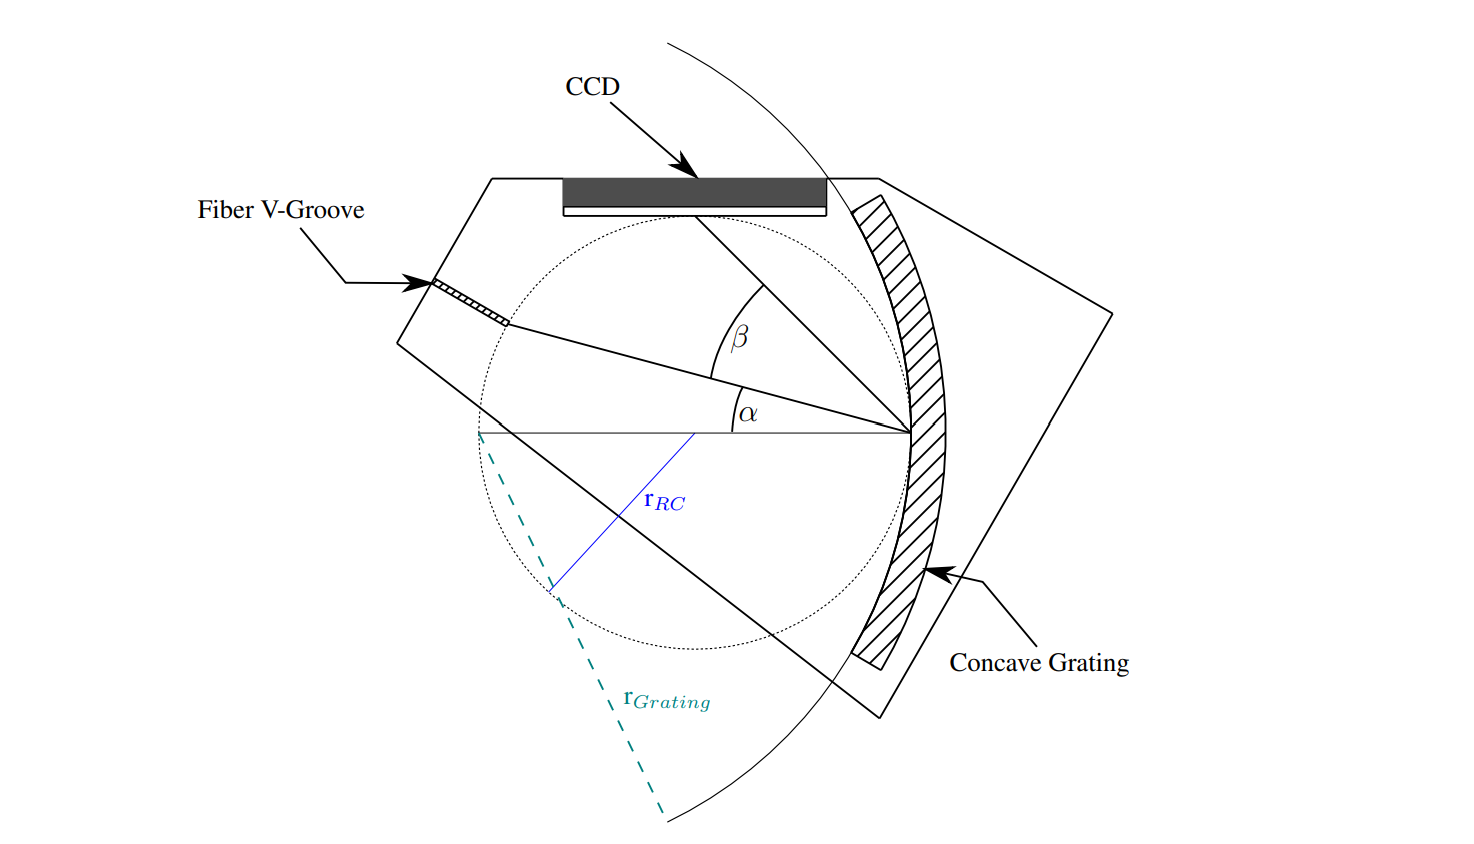
\includegraphics{/images/grating_diagram_dd.png}}
%\includegraphics{/images/proposal_layout.pdf_tex}
%\caption{\label{fig:spec_intro}Spectrometer grating layout.}
\end{figure}

\newpage

\section{Introduction and Background}

\subsection{Basis for Design}
The foundational work for this design comes from P. Pottier et al. \cite{Packirisamy2012Mono-OrderGrating}. The reference design, is displayed in Figure \ref{fig:pot_ref}, the left image is a traditional planar Rowland grating, whereas the right is a mono-order distributed Bragg reflector grating. The design presented in this report follows the latter, as it offers greater efficiency than the traditional grating, and its construction lends itself to programmatic generation. 

\begin{figure}[H]        
\centering
\scriptsize 
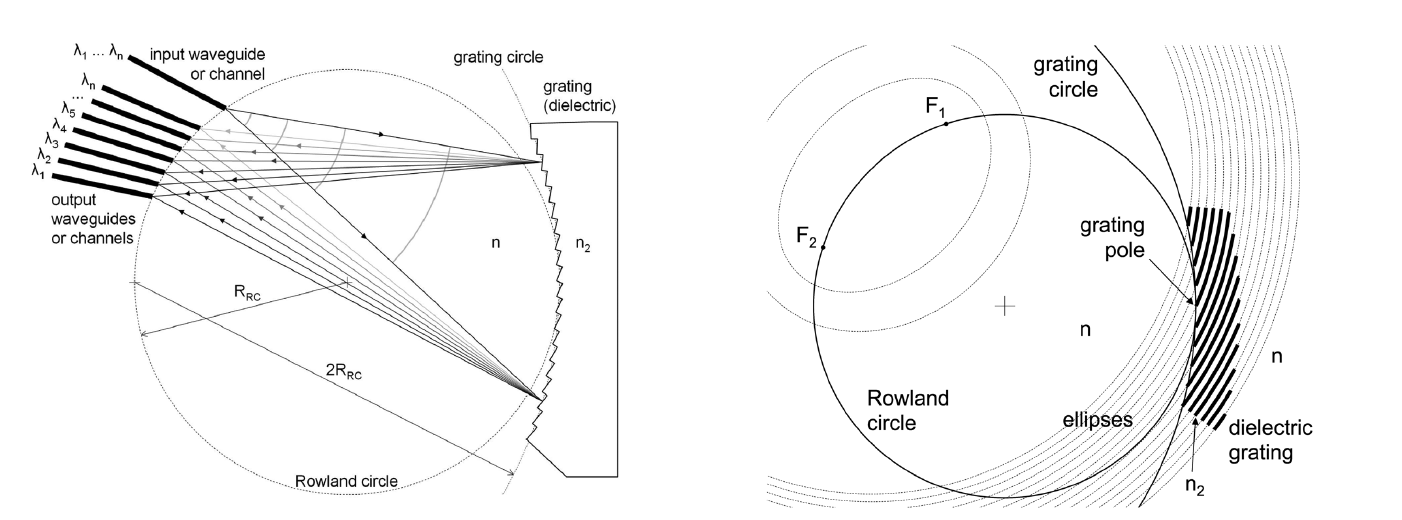
\includegraphics[width=0.9 \textwidth]{/images/pottier.png}
\caption{\label{fig:pot_ref} Reference grating geometries, reproduced from from P. Pottier et al. \cite{Packirisamy2012Mono-OrderGrating}.}
\end{figure}

\begin{figure}[H]
\centering
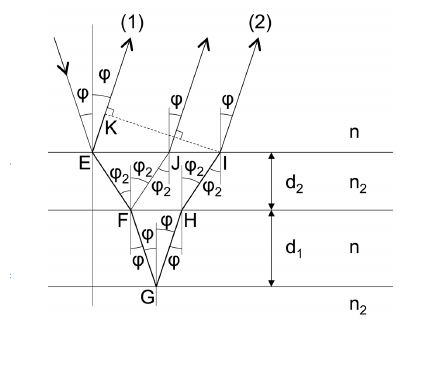
\includegraphics[width=0.65\textwidth]{/images/bragg_cond.png}
\caption{ Bragg condition for two material stack \cite{Packirisamy2012Mono-OrderGrating}.}
\label{fig:nanos_test_code0}
\end{figure}

\subsection{Verification of Elliptical Design}
The following equations describe the various geometrical and optical condition for optimal device performance \cite{Packirisamy2012Mono-OrderGrating,Pottier2014IntegratedInsulator}. As discussed in the work of P. Pottier et al. \cite{Packirisamy2012Mono-OrderGrating}, drawing ellipsis who's foci are the input and output points with thickness \(d_2\) offset from one another by a distance $d$ (the center to center distance), satisfies the diffraction conditions and the blazing condition. However, as discussed below, the bragg reflector stack cannot be fabricated in an ideal manner. Despite this, if the ellipse thickness is much smaller than the spacing between the ellipsis, that is $\frac{d_2}{d} \approx 0$, the device's efficiency is maximized.

\subsubsection{Equations}

To improve the device's efficiency, the grating may be curved. The radius of the grating must be $2 R_{RC}$, so that it focuses the input light into the outputs placed around the Rowland Circle. It's worth noting that the radius does not particularly matter, for the purposes of this design
\begin{equation}
    \vb{M \lambda} = - n a (\sin{\alpha} + \sin{\beta})
    \label{eq:a}
\end{equation}
                We also note, 
\begin{equation*}
    \sin{\theta} = \frac{d}{a}
\end{equation*}
                
The second diffraction condition comes from finding the path length difference $\delta$,
\begin{equation*}
    m \lambda = 2 \Bigg[ n d_1 \cos{\phi} + n_2 d_2 \sqrt{1-(\frac{n}{n_2})^2 \sin^2 \phi} \Bigg]
\end{equation*}

To select our pass-band center, the angle of the grating lines with respect to the grating normal, $\phi$, should obey Snell's law. That is,

\begin{equation*}
    \left \lbrace
    \begin{aligned}
        &\alpha - \phi + \theta = 0\\
        &\alpha - \beta = 2 \phi\\
    \end{aligned}
    \right.
\end{equation*}

Rearranging the above conditions yield the following critical relation, so if $a$ is found using equation \ref{eq:a}, the center-to-center distance $d$ is
\begin{equation}
d = -a \sin (\frac{\alpha + \beta}{2})
    \label{eq:d}
\end{equation}

The optimal Bragg reflector dimensions are
\begin{equation*}
    \left \lbrace
    \begin{aligned}
        &d_1 = \frac{(2 k_1 +1) \lambda}{4 n \cos{\phi}}\\
        &d_2 = \frac{(2 k_2 +1) \lambda}{4 n_2 \cos{\phi_2}}\\
        &k_1, k_2 \in \mathbb{Z}
    \end{aligned}
    \right.
\end{equation*}
It is very difficult to select dimensions such that the above conditions are met; however, if $\frac{d_2}{d} \approx 0$ or $d_1 = d_2$ and $n_2 \approx  n$ then the path length difference from both conditions is approximately equal \cite{Packirisamy2012Mono-OrderGrating, Pottier2014IntegratedInsulator}. Therefore $m=-M$, which optimizes device efficiency.


\section{Implementation}
    The entirety of the design work takes place in the python programming language; specifically, using the geometric package Shapely. Shapely is a BSD-licensed Python package for manipulation and analysis of planar geometric objects \cite{ShapelyDocumentation}. The key advantage of using shapely to define photonic circuit elements is the native support for gdshelpers, another package which takes shapely polygons and curves and generates photonic devices \cite{WelcomeDocumentation}. From MZIs, waveguides, couplers, and resonators the gdshelper package offers many tools for creating GDSII files, which are standard for lithography tools. Furthermore, the open source FDTD package, Meep, offers a GDSII importer for simulations \cite{ManualDocumentation}. Although I did not generate mask files or simulate the structure, which is discussed further below, it is possible to implement the closed-loop algorithm in Figure \ref{fig:alg} entirely in one script.

    
    
    \subsection{Algorithm}
    
    \begin{figure}[H]        
    \centering
    \scriptsize 
    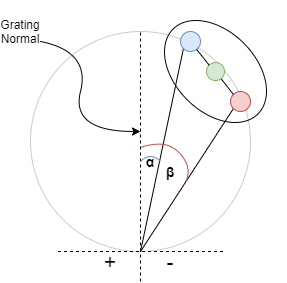
\includegraphics[width=0.5\textwidth]{/images/grating_construction.png}
    \caption{\label{fig:grating_angles} Grating geometric construction, the blue point is the input waveguide, the red point is the center of the output band, and the green point is the ellipse center. Also shown is the grating angle sign convention, an angle in the first quadrant is negative.}
    \end{figure}
    
    For the geometry configuration in Figure \ref{fig:grating_angles}, after solving the ellipse offset, d, in Equation \ref{eq:d}, the grating ellipsis are generated with the following code 
\lstset{caption={Ellipse Class}}
\begin{lstlisting}
class GratingEllipse(ParametricGeometry):
    max_radius = 0

    def __init__(self, focus_0, focus_1, offset=0, origin=None):
        super().__init__(origin)
        A, B = (focus_0.u, focus_0.v), (focus_1.u, focus_1.v)
        # x axis angle, needed for ellipse orientation
        theta = atan2(B[1]-A[1], B[0]-A[0])  
        center = focus_0.midpoint(focus_1)
        self.u, self.v = center[0], center[1]
        
        
        foci_spacing = sqrt((B[1]-A[1])**2 + (B[0]-A[0])**2)
        major_axis = foci_spacing+2*offset
        minor_axis = sqrt(major_axis**2-foci_spacing**2)
        from shapely import affinity
        
        # create a circle of radius 1
        curve = Point(self.u, self.v).buffer(1)
        # create the ellipse by scaling the circle along x and y:
        curve = affinity.scale(curve, major_axis, minor_axis)
        
        # Rotate the ellipse (clockwise, x axis pointing right):
        self.curve = affinity.rotate(curve, theta, use_radians=True).boundary
\end{lstlisting}
    The final remaining unknown variable is the Rowland radius. The actual value of the radius does not impact device performance so long as the radius is greater than a few microns and the input beam divergence is relatively small \cite{Packirisamy2012Mono-OrderGrating}. For example, the spectra in Figure \ref{fig:ref_spec} are produced by a device with $R_{RC} = 50 \ \mu m$. Given this freedom, and that the linear dispersion scales directly with the radius of a concave grating, $R_{RC}$ should be scaled to fit the free spectral range of the device. However, there is no empirical equation for the FSR because the Bragg reflector limits the pass band. Figure \ref{fig:ref_spec} illustrates this by simulating an identical structure with varying reflector dimensions.
    
    Figure \ref{fig:alg} illustrates how FDTD may be leveraged to generate the optimal geometry for our device. However, because the Heidelberg maskless aligner in MRL has a minimum feature size of 600 nm, multiple exposures are required to meet the $\frac{d_2}{d} \approx 0$ approximation. This requirement means that the GDSII files for simulation and fabrication must be different; ultimately, I chose to simply define the elliptical curves so I could use them as a scaffold for both patterns.

    \begin{figure}[H]        
    \centering
    \scriptsize 
    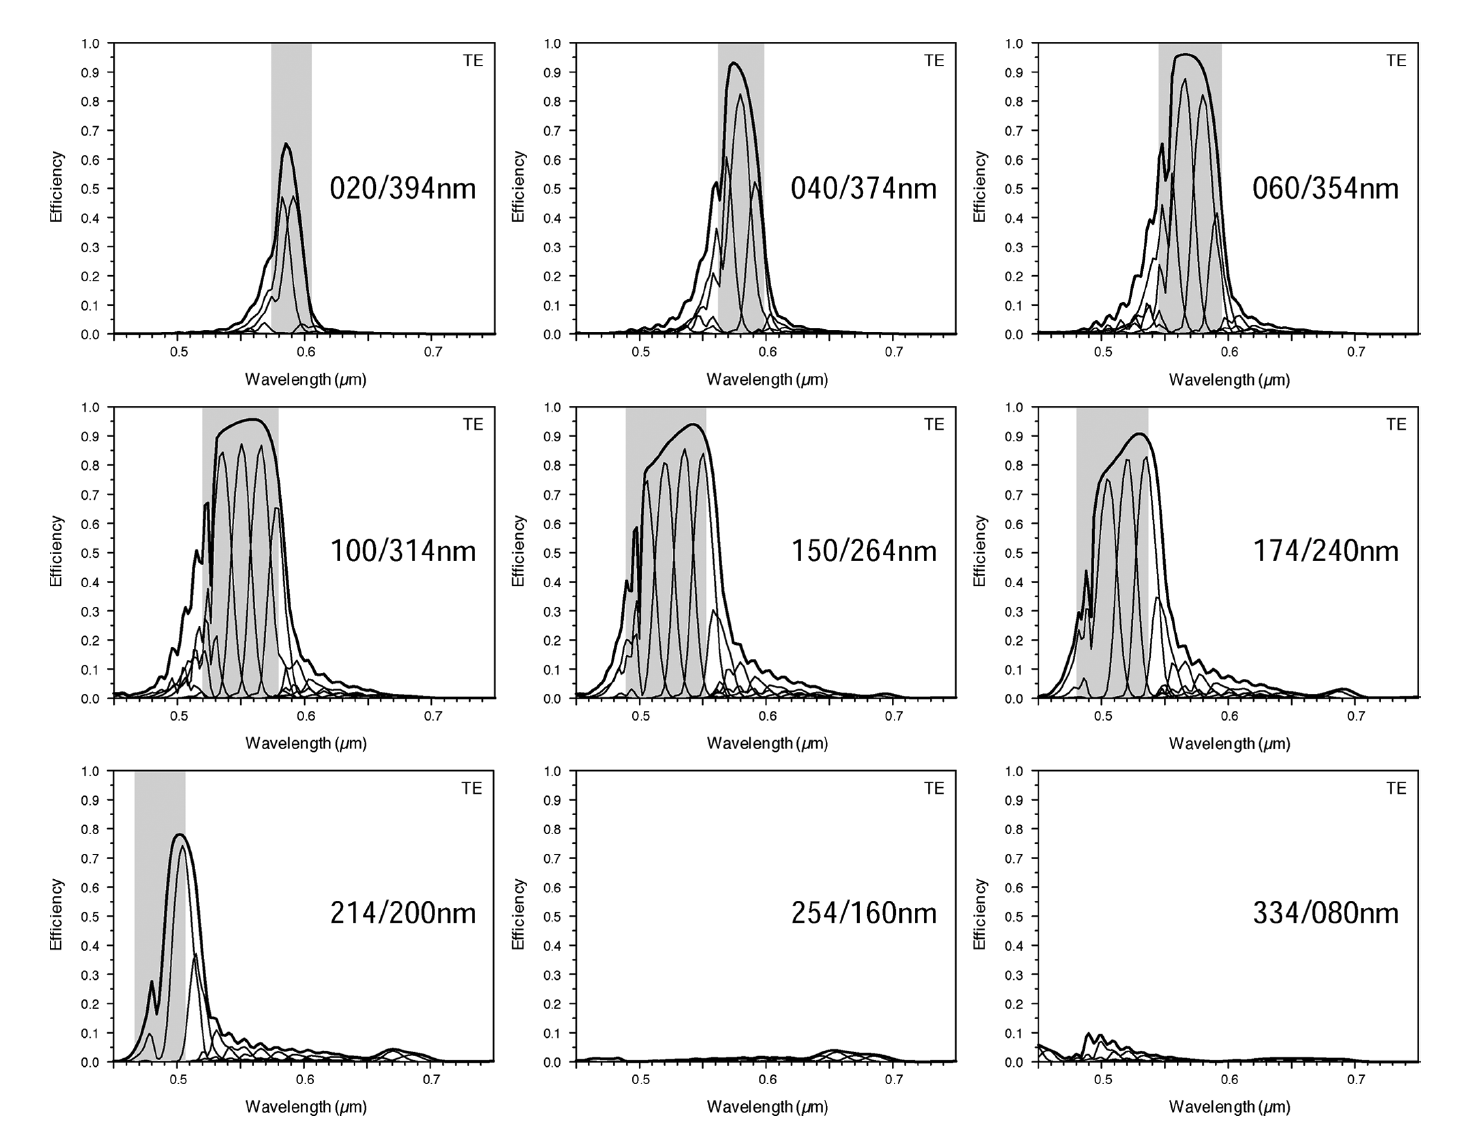
\includegraphics[width=0.7\textwidth]{/images/ref_simulation.png}
    \caption{\label{fig:ref_spec} Grating spectrum for varying values of $\frac{d_2}{d}$. The bandwidth of the system is bound by the bragg reflector, not the grating itself. Reproduced from from P. Pottier et al. \cite{Packirisamy2012Mono-OrderGrating}.}
    \end{figure}

    \begin{figure}[H]        
    \centering
    \scriptsize 
    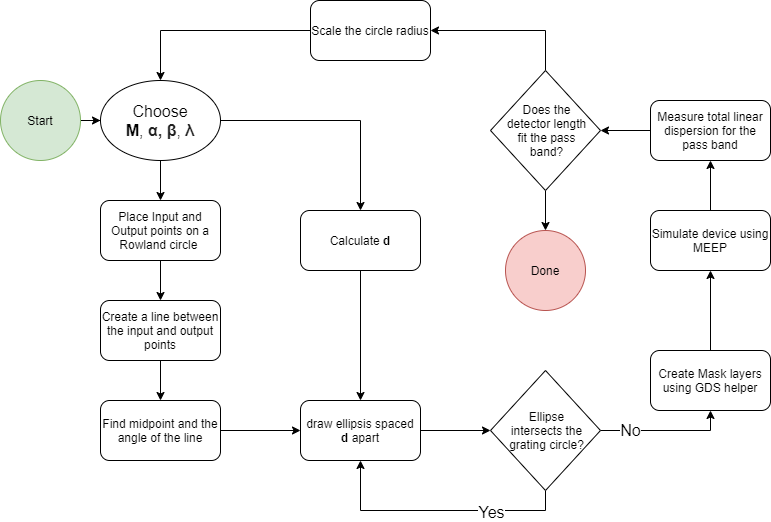
\includegraphics[width=0.8\textwidth]{/images/grating_algorithm.png}
    \caption{\label{fig:alg} Grating construction algorithm, .}
    \end{figure}
    
    \subsection{Remaining Work}
    Unfortunately, the only FDTD experience I have is from this class, so I wasn't able to get the simulations running in this short amount of time. As previously discussed, because the masks for fabrication and simulation must be different I was reluctant to make my script geared towards a single application. To compromise, the ellipsis are defined by a center line, which shapely easily can buffer a polygon around. 
    
    Ultimately, I still plan to use my experience with microelectronics to fabricate a low-cost spectrometer for my applications. In particular, I am starting my PhD at UIUC next semester, and I would like to add several spectrometers to my reaction chamber. I have spent the last two years developing a python to python/c++ compiler for creating closed loop processing of semiconductors; however, I do not have a characterization device built on the same framework. If you are interested in the future development of my software my GitHub is \url{https://github.com/LukasJanavicius}, though note that the compiler has not been published for release at this time. 


    \subsection{Discussion}
    I have elected to omit code (with the exception of the ellipsis) from this report for the sake of brevity, but I will provide it alongside my submission. Feel free to use any of the material from this report or the script for future use. Given that gdshelpers has built in tools for generating MZI structures with grating couplers \cite{WelcomeDocumentation}, perhaps someone could implement their silicon photonics lab using this script and actually test the device. 
    
    I did not have time to completely generate the necessary files for the device; however, I wrote an auxiliary plotting script which accepts a parameter name and a range of values. Note that only one parameter is varied at a time, and the others are held constant at their value in Table \ref{tab:std_param}.
    
    \begin{table}[H]
    \centering
    \caption{Standard grating configuration parameter, unless otherwise specified these parameters are held constant throughout the construction. Also, note that the unit of the Rowland circle and grating thickness is arbitrary, and may be assigned when writing to a GDSII helper.}
    \label{tab:std_param}
    \begin{tabular}{|l|l|l|l|l|l|l|l|}
    \hline
    $n$ & $n_2$ & $\lambda_{grating}$ & M  & $\alpha$      & $\beta$       & $R_{RC}$ & $t_{grating}$ \\ \hline
    1.5 & 1     & 600 nm              & -2 & -15$^{\circ}$ & -45$^{\circ}$ & 10       & 3             \\ \hline
    \end{tabular}
    \end{table}
    
    
\section{Results}


    \begin{figure}[H]        
    \centering
    \scriptsize 
    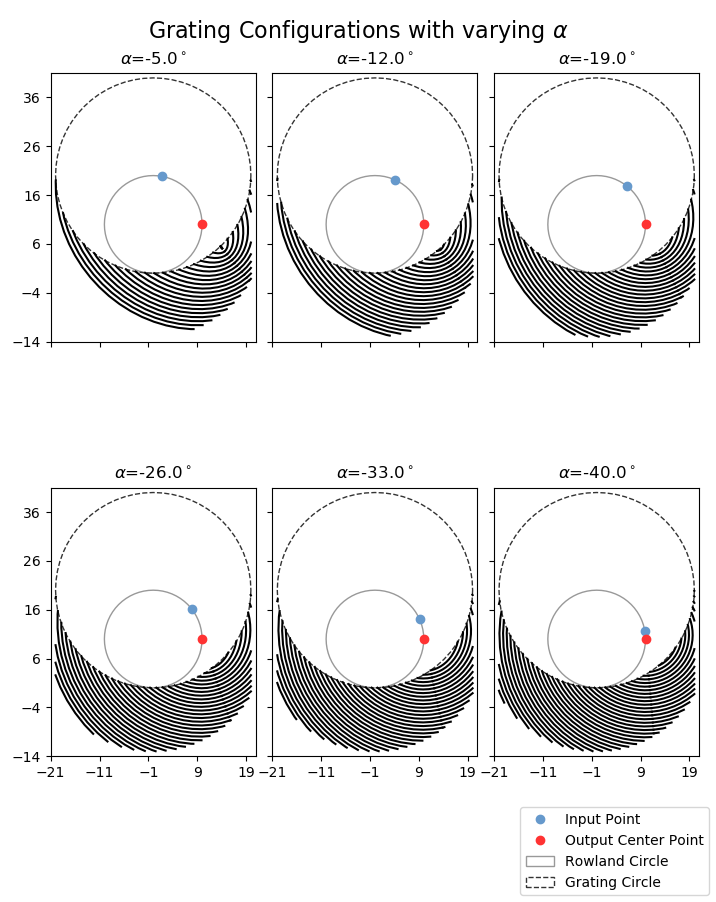
\includegraphics[width=0.9 \textwidth]{/images/varied_alpha_0.png}
    \caption{\label{fig:vary_alpha} Grating geometries with varying input angle. Note the eccentricity of the ellipsis at large angle differences, and the circularity when approaching the Littrow condition $\alpha = \beta$.}
    \end{figure}
    
    \begin{figure}[H]        
    \centering
    \scriptsize 
    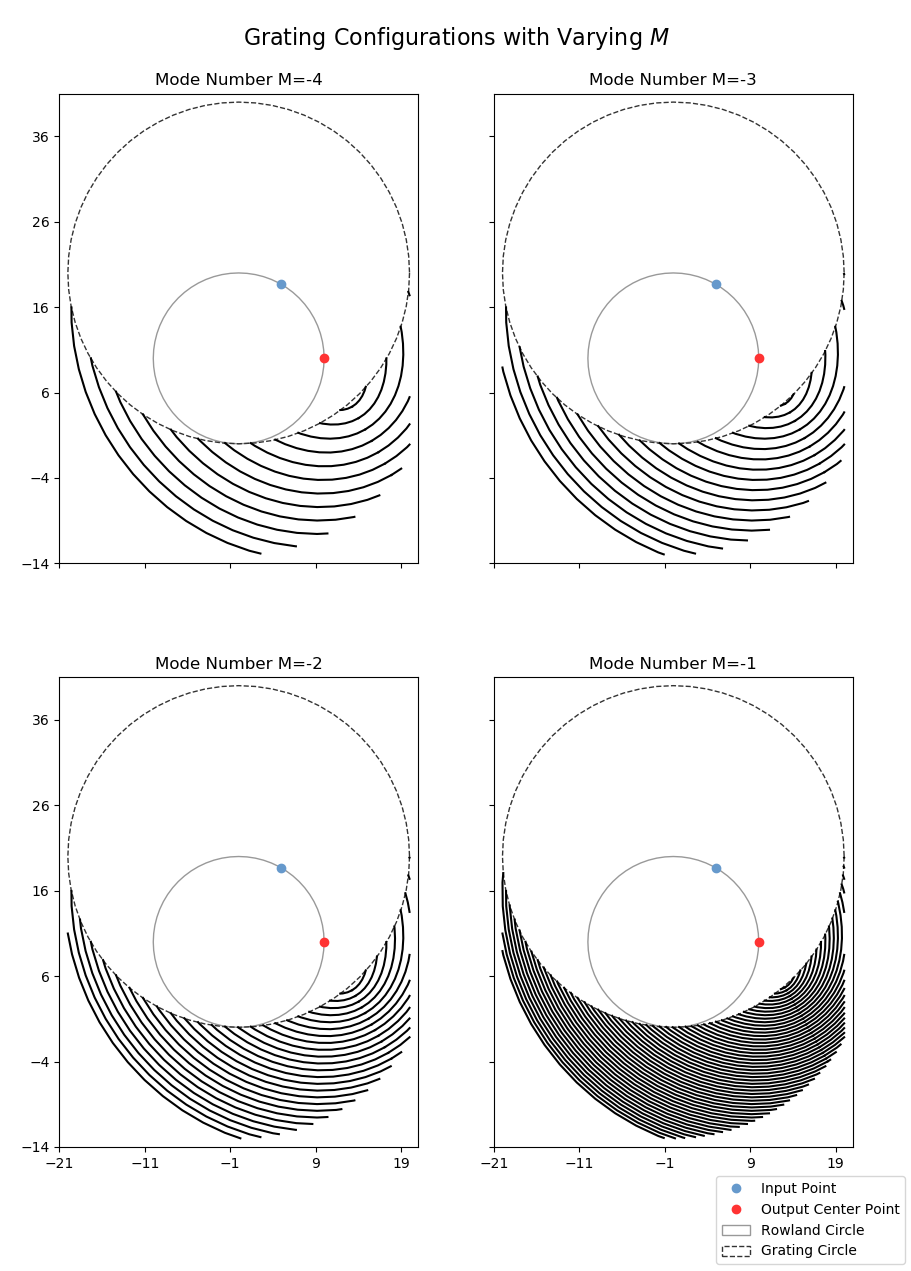
\includegraphics[width=0.9 \textwidth]{/images/varied_M_0.png}
    \caption{\label{fig:vary_M} Grating geometries with varying mode number $M$. As M decreases so does the grating spacing.}
    \end{figure}
    
    \begin{figure}[H]        
    \centering
    \scriptsize 
    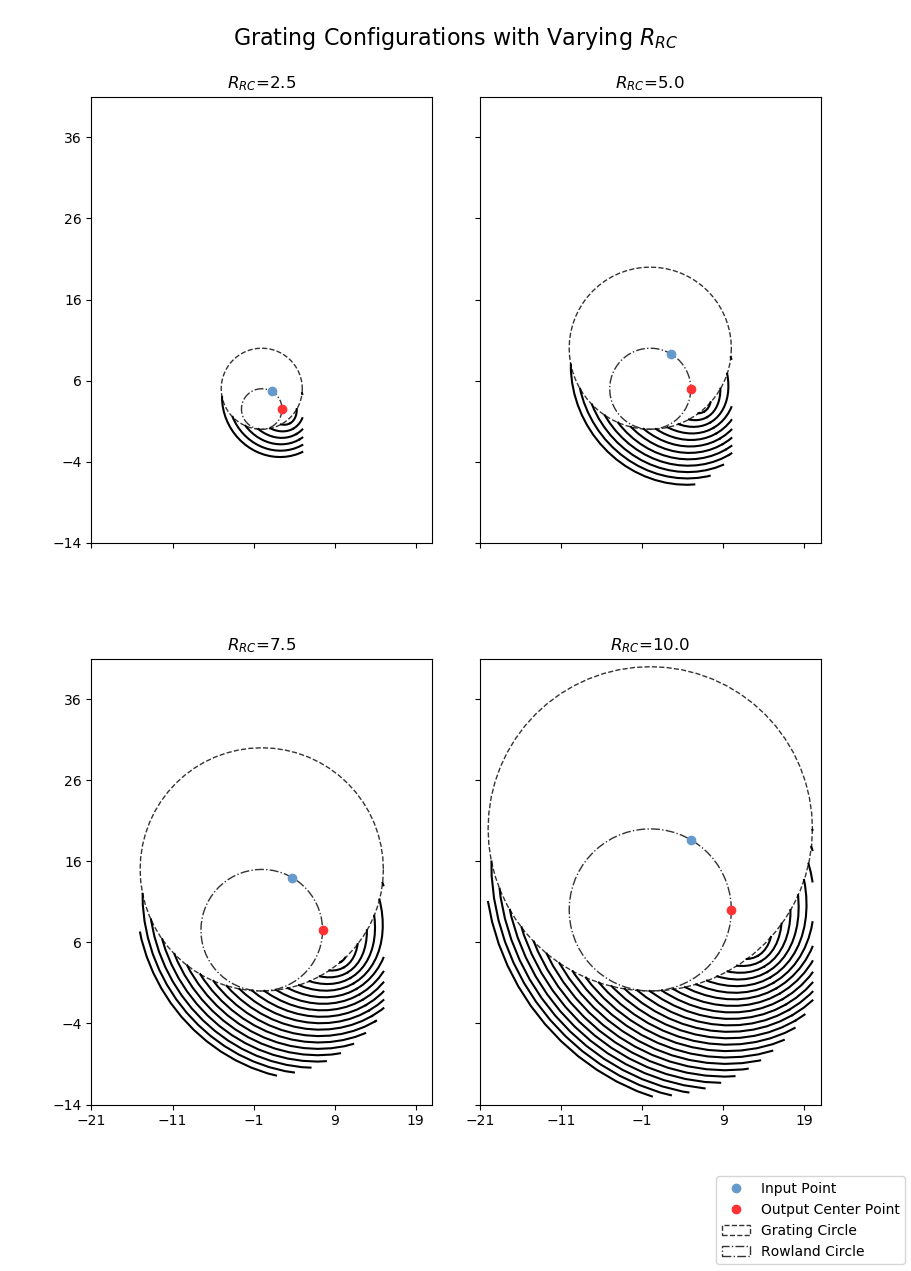
\includegraphics[width=0.9 \textwidth]{/images/vary_r.png}
    \caption{\label{fig:vary_R} Grating geometries with varying Rowland radius. Grating spacing is independent of $R_{RC}$.}
    \end{figure}
    
     \begin{table}[H]
    \centering
    \caption{Grating spacing as a function of the input angle.}
    \label{tab:d_vs_alpha}
    \begin{tabular}{|l|l|}
    \hline
    $\alpha$ & d (nm)  \\ \hline
    -5.0     & 389.568 \\ \hline
    -12.0    & 386.191 \\ \hline
    -19.0    & 382.462 \\ \hline
    -26.0    & 378.487 \\ \hline
    -33.0    & 374.392 \\ \hline
    -40.0    & 370.314 \\ \hline
    \end{tabular}
    \end{table}
    
    \begin{table}[H]
    \centering
    \caption{Grating spacing as a function of M.}
    \label{tab:vary_m}
    \begin{tabular}{|l|l|}
    \hline
    M  & d (nm)  \\ \hline
    -4 & 769.26  \\ \hline
    -3 & 576.945 \\ \hline
    -2 & 384.63  \\ \hline
    -1 & 192.315 \\ \hline
    \end{tabular}
    \end{table}
    
    \subsection{Discusssion}
    Although my script can vary the grating geometry for any parameter in Table \ref{tab:std_param}, Figures \ref{fig:vary_alpha} through \ref{fig:vary_R} are meant to illustrate the geometry's dependence on parameters which may be freely chosen. The indices of refraction and target wavelength are bound by the material system and application, so are held constant for my purposes. 
    
    Tables \ref{tab:d_vs_alpha} and \ref{tab:vary_m} show how the design may be tweaked to fit lithographic constraints either by angle or mode number. It is worth noting that, as with a traditional spectrometer, with increasing $\abs{M}$ the device's resolving power increases, but the free spectral range decreases. For my applications I would like the greatest FSR possible, but as Figure \ref{fig:vary_M} illustrates, low mode numbers require extremely tight patterns. Using the school's photolithography tools I would expect to achieve a minimum $\abs{M} = 4$, and with a dedicated mask it should be possible to achieve $\abs{M} = 2$. Without simulations or empirical equations for the device's resolving power or FSR I cannot comment on their expected values. However, given the side wall roughness produced when fabricating photonics I fully confident my device's efficiency will by much lower than that reported by P. Pottier et al. \cite{Packirisamy2012Mono-OrderGrating}.
    
\clearpage
\newpage
\bibliographystyle{IEEEtran}
\bibliography{bibliography/references}

\addcontentsline{toc}{section}{References}
\end{document}
